\chapter{Snímky dokumentace}

\section{Úvodní obrazovka}

\begin{figure}[H]
  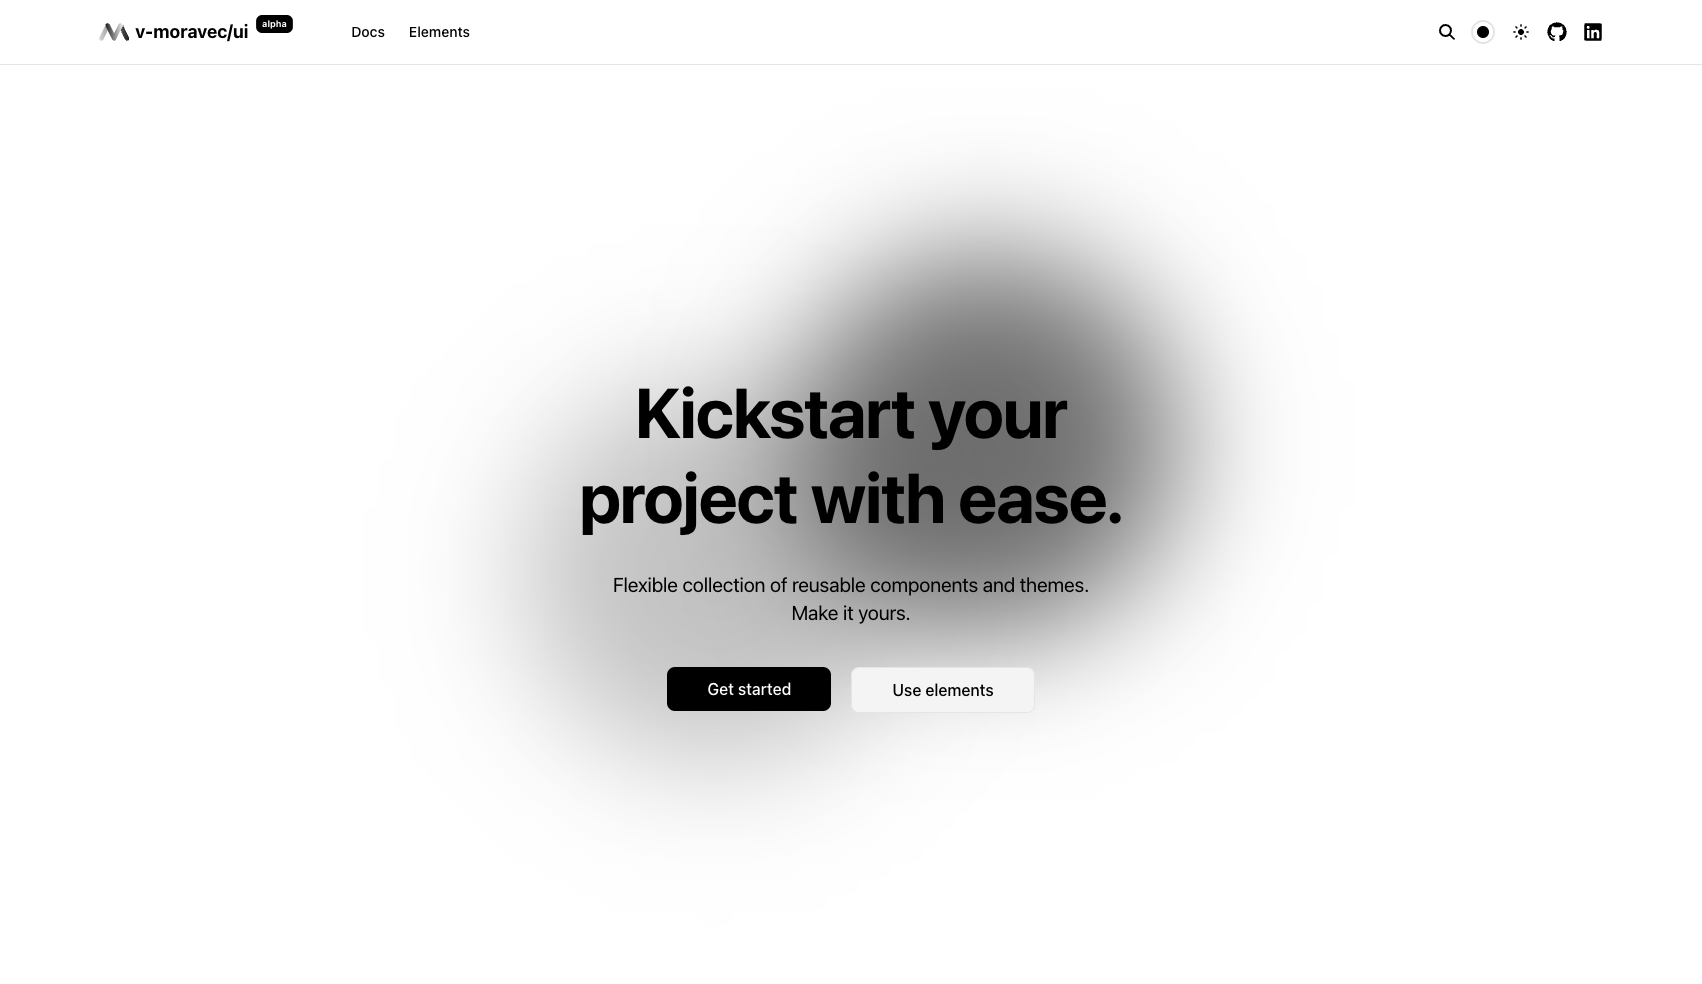
\includegraphics[width=\textwidth]{images/main-page}
  \caption{Úvodní obrazovka} \label{picture:documentation:main-page}
\end{figure}

\begin{figure}[H]
  \centering
  \subfloat[Tmavá verze]{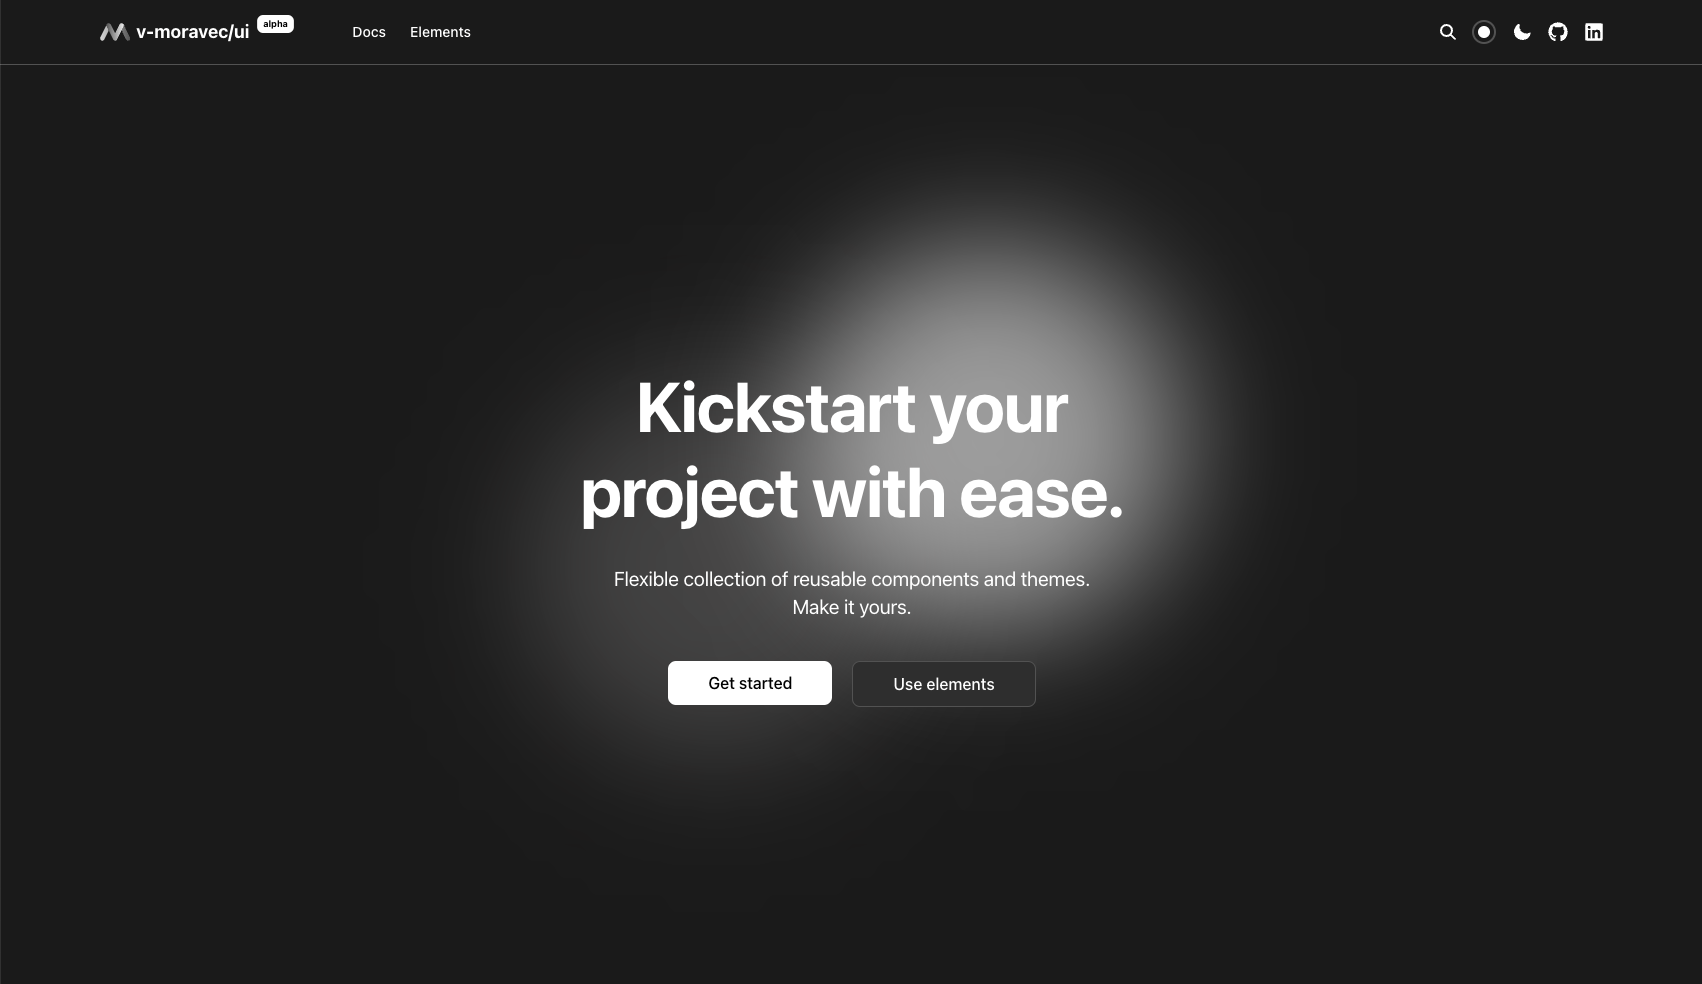
\includegraphics[width=0.3\textwidth]{images/main-page-dark}\label{picture:documentation:main-page-dark}}
  \subfloat[Modrá verze]{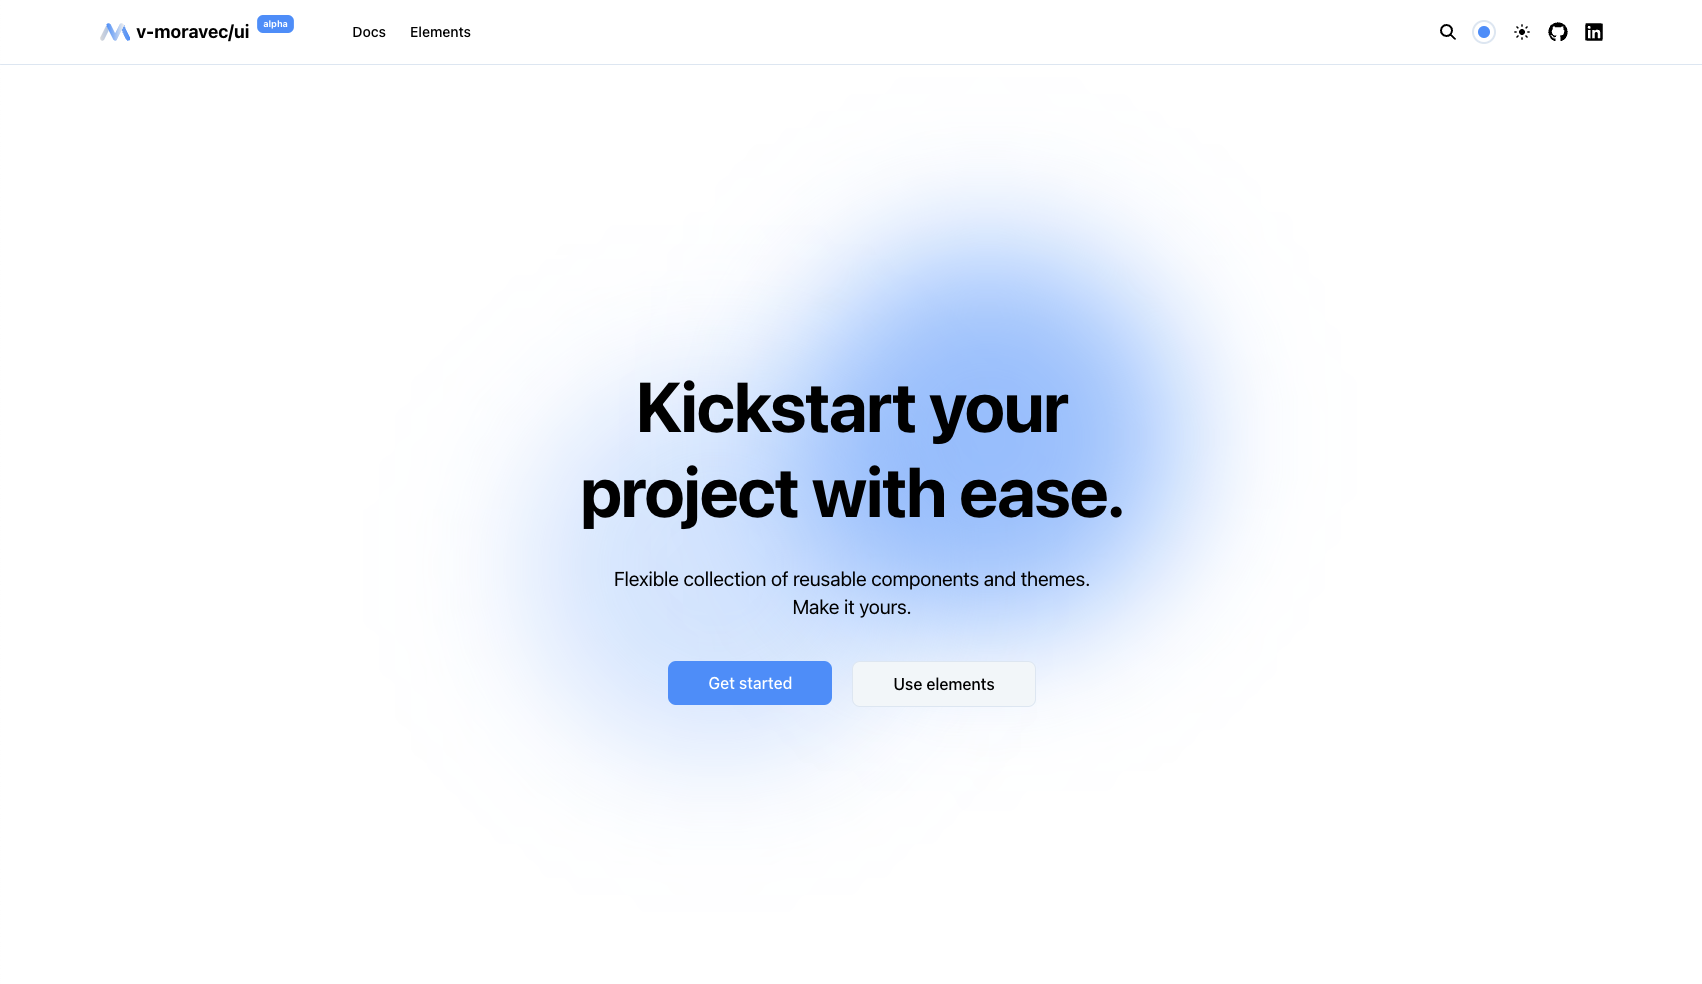
\includegraphics[width=0.3\textwidth]{images/main-page-colored}\label{picture:documentation:main-page-colored}}
  \caption{Stylování}
\end{figure}

\section{Komponenty}

\begin{figure}[H]
  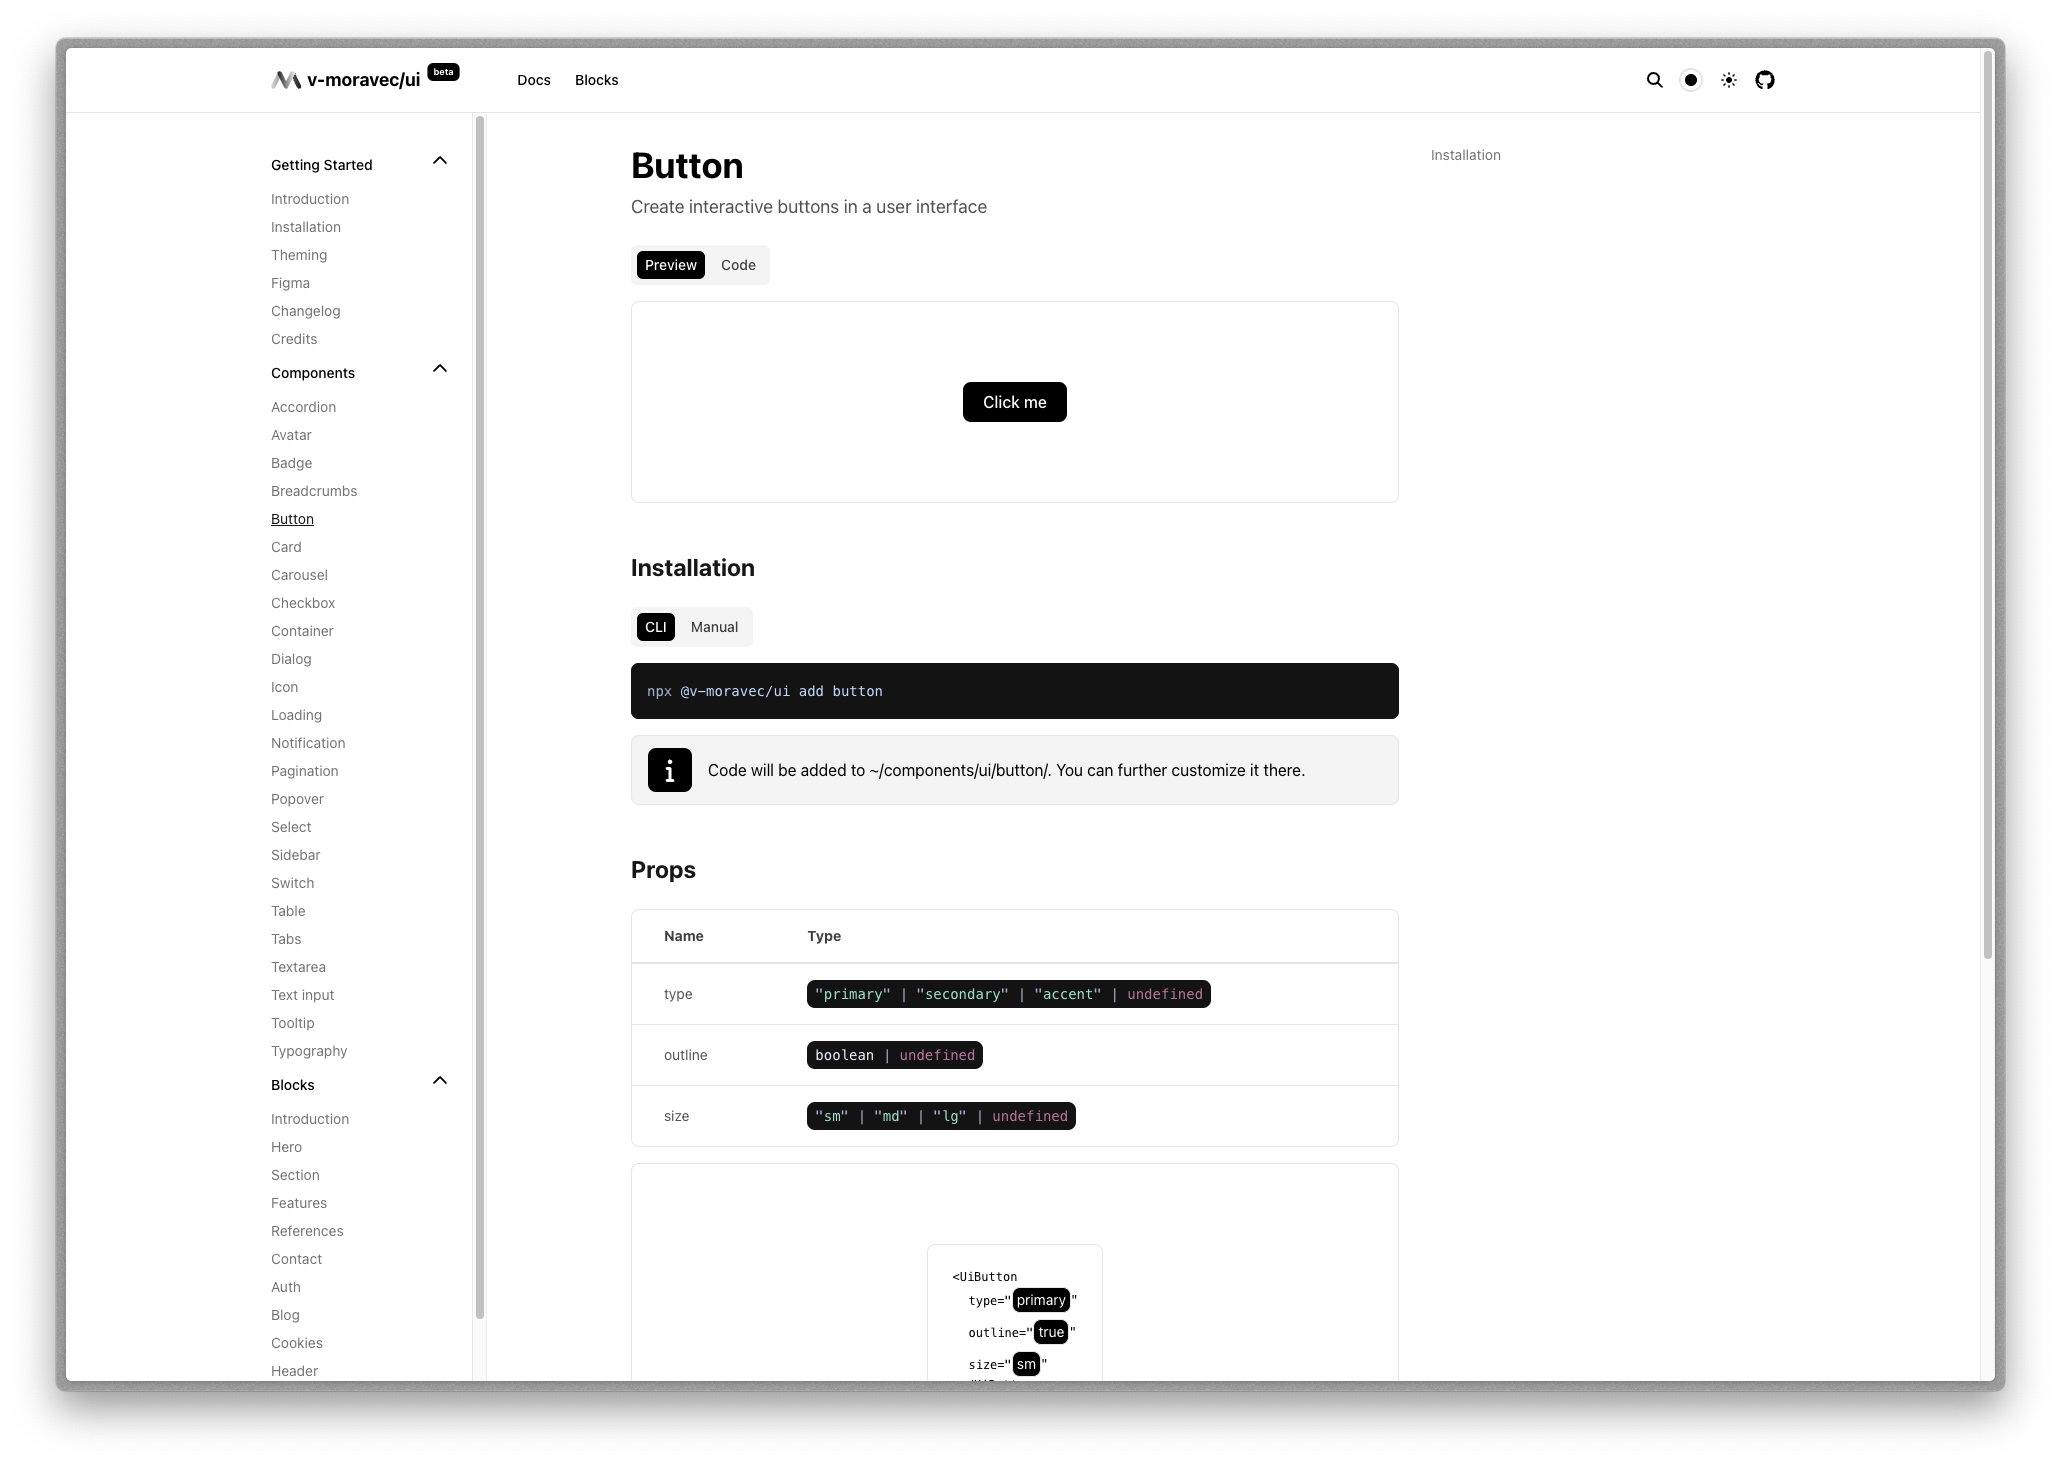
\includegraphics[width=\textwidth]{images/component-preview}
  \caption{Zobrazení komponenty} \label{picture:documentation:component-preview}
\end{figure}

\begin{figure}[H]
  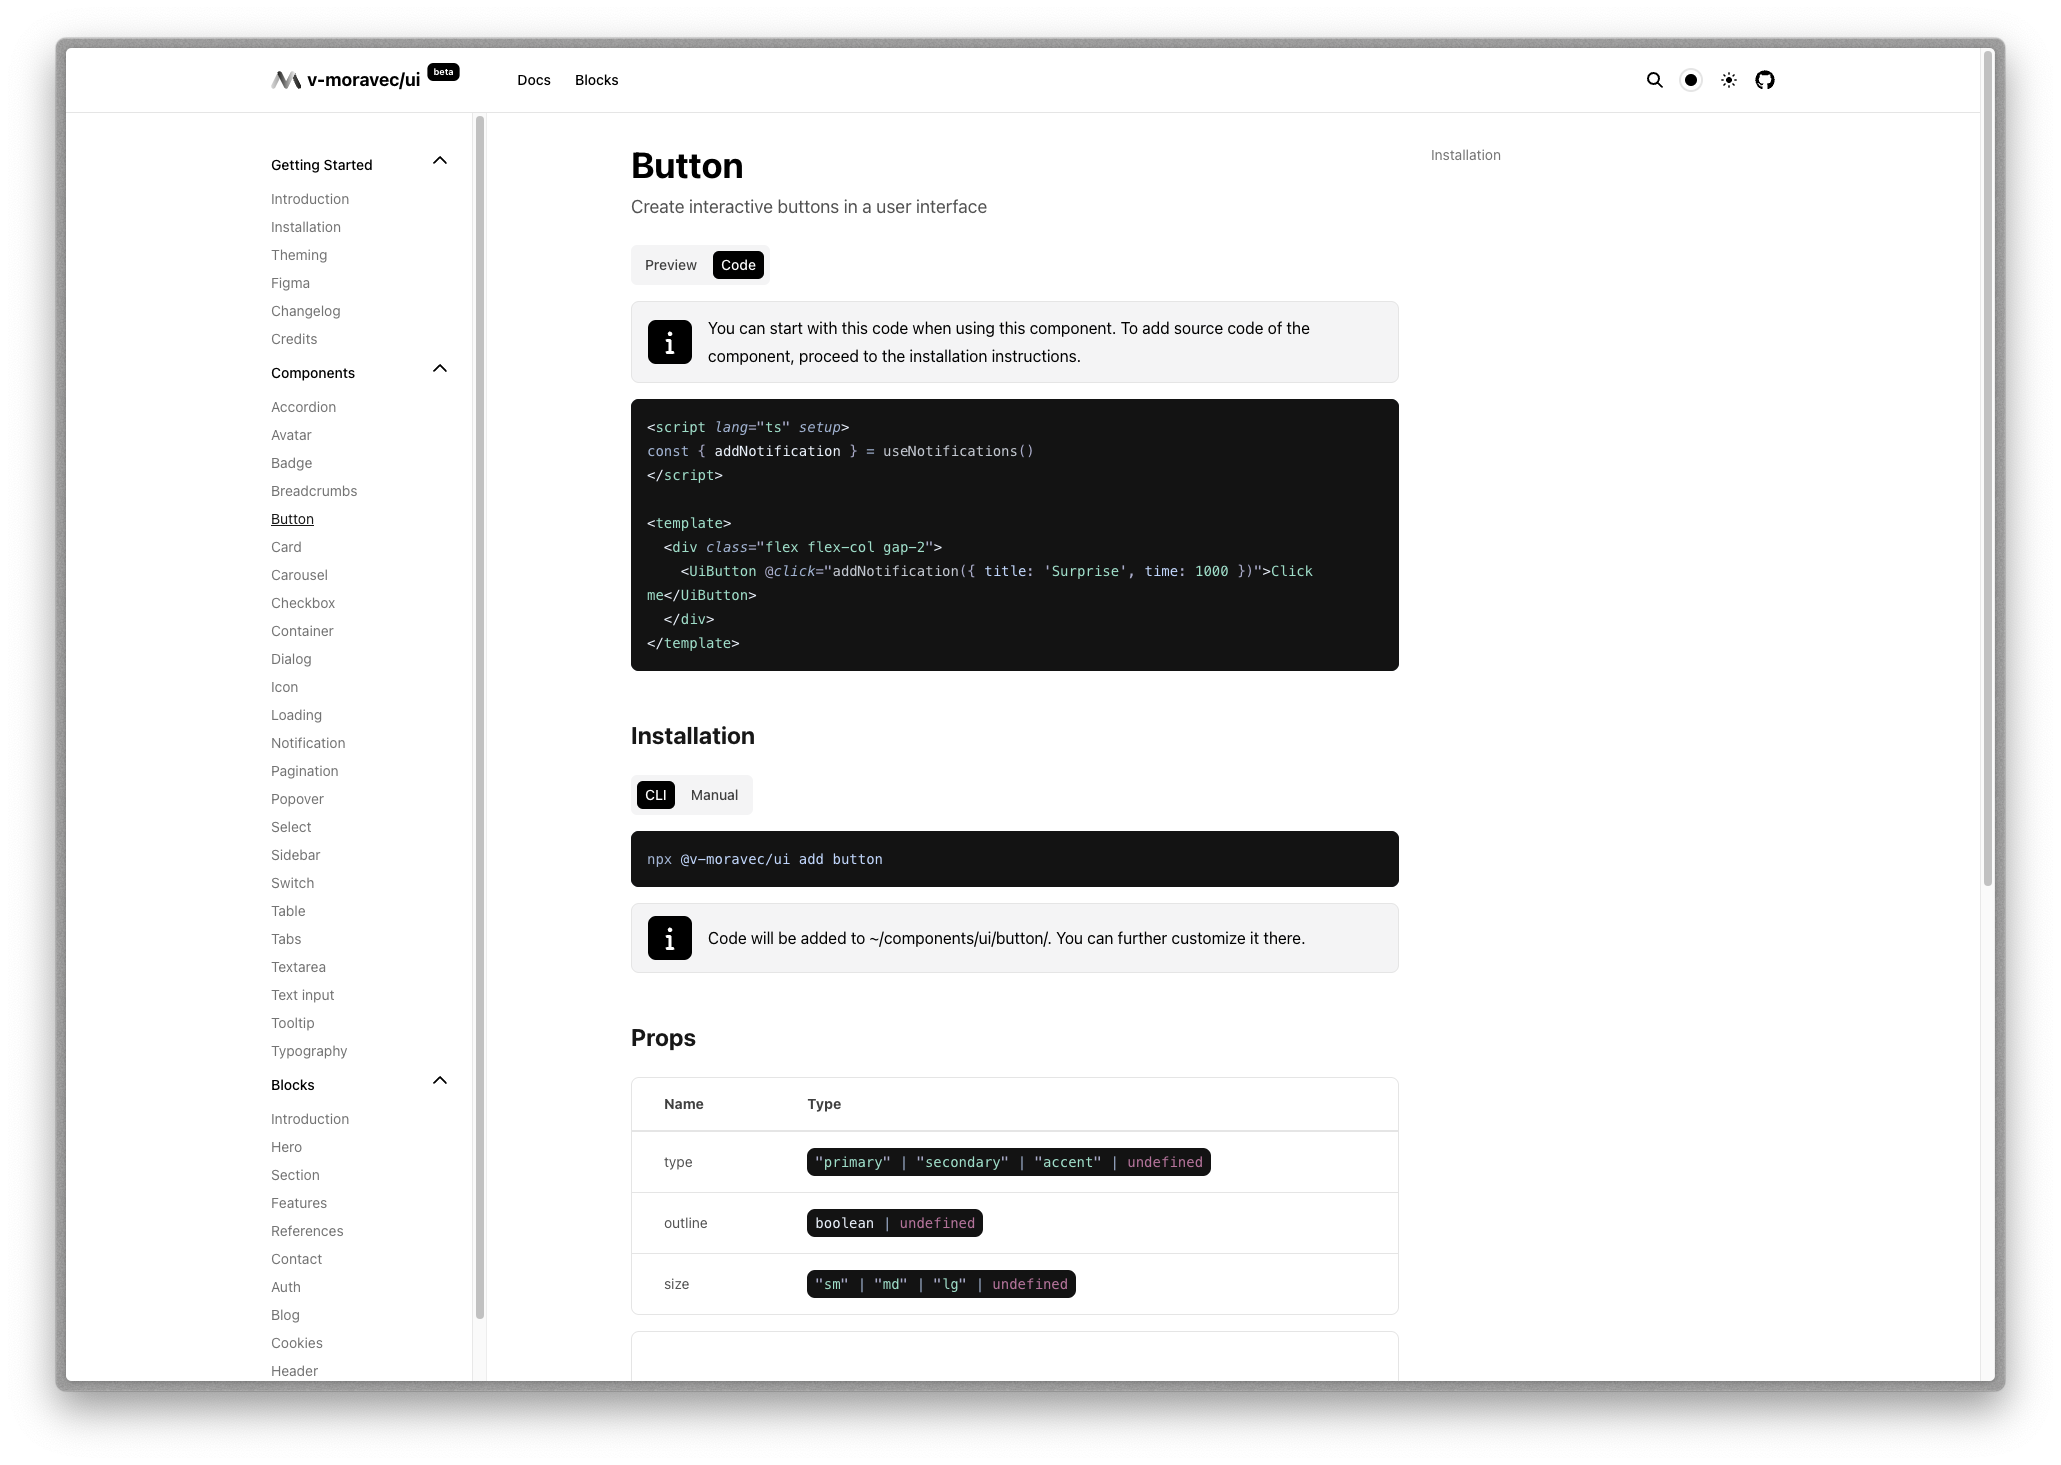
\includegraphics[width=\textwidth]{images/component-code}
  \caption{Kód komponenty} \label{picture:documentation:component-code}
\end{figure}

\section{Elementy}

\begin{figure}[H]
  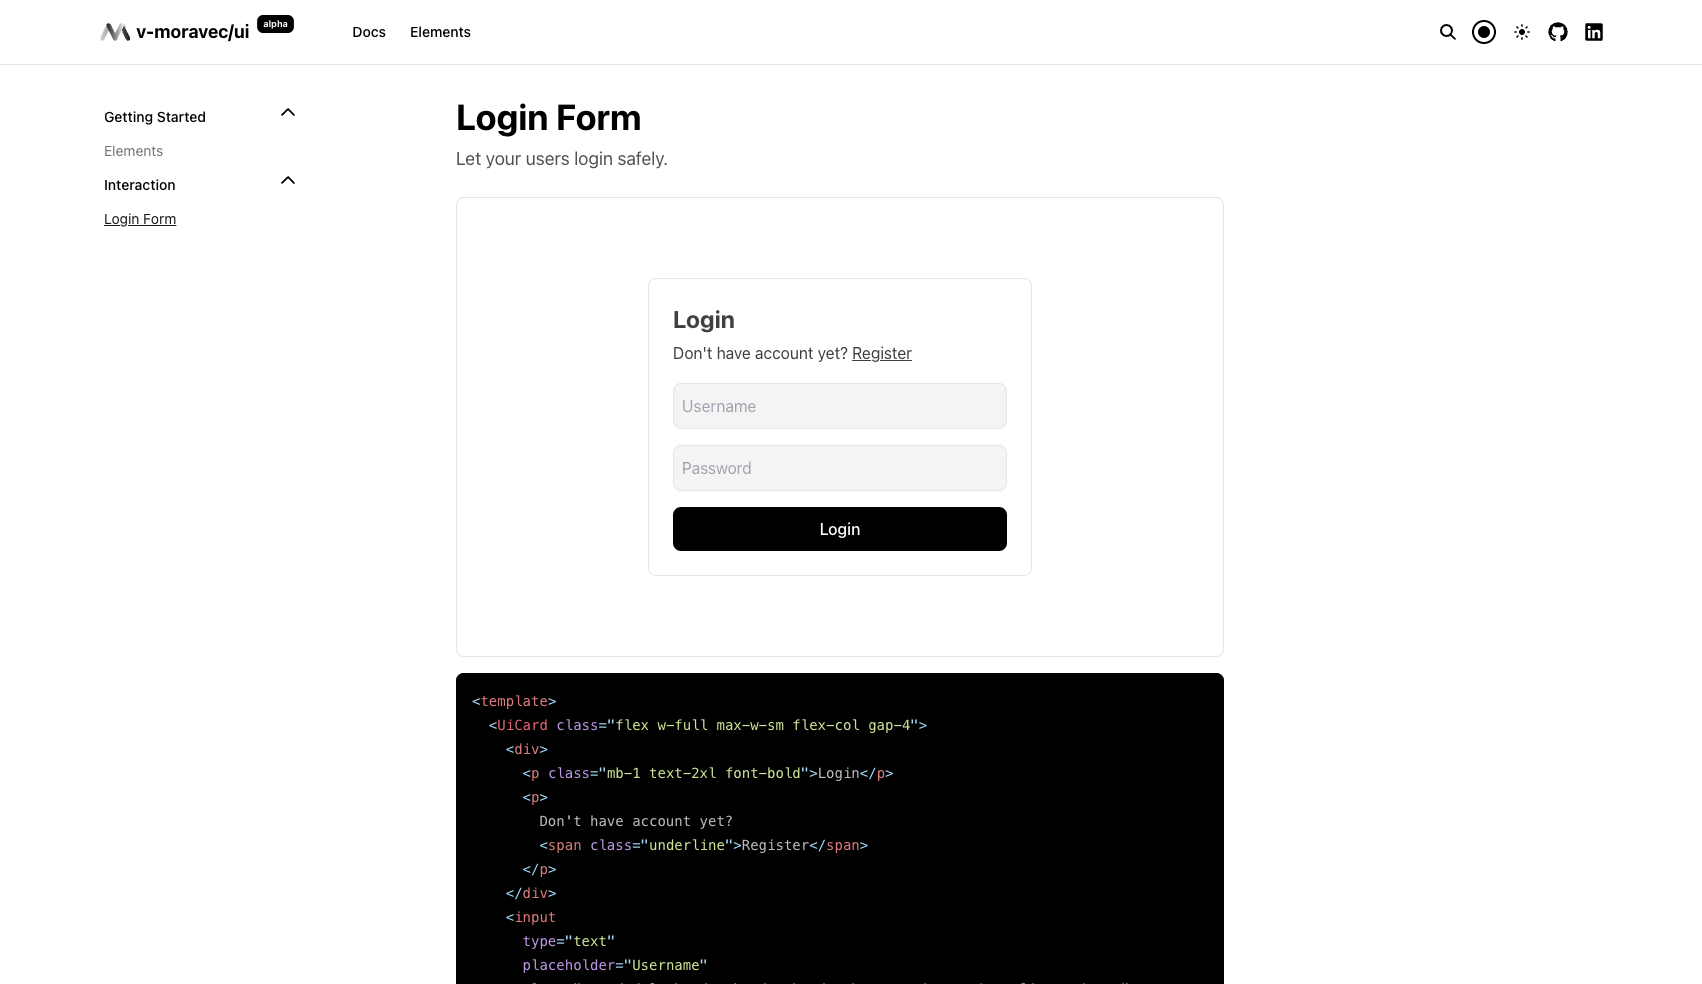
\includegraphics[width=\textwidth]{images/element}
  \caption{Element složený z komponent} \label{picture:documentation:element}
\end{figure}
